\documentclass{beamer}
\usepackage[utf8]{inputenc}
\usepackage{graphicx, epsfig}
\usepackage{amsmath,mathrsfs,amsfonts,amssymb}
\usepackage{floatflt}
\usepackage{epic,ecltree}
\usepackage{mathtext}
\usepackage{fancybox}
\usepackage{fancyhdr}
\usepackage{multirow}
\usepackage{enumerate}
\usepackage{epstopdf}
\usepackage{multicol}
\usepackage{algorithm}
\usepackage[noend]{algorithmic}
\usepackage{tikz}
\usepackage{blindtext}
\usetheme{default}%{Singapore}%{Warsaw}%{Warsaw}%{Darmstadt}
\usecolortheme{default}

\setbeamerfont{title}{size=\Huge}
\setbeamertemplate{footline}[page number]{}

\setbeamertemplate{section in toc}[sections numbered]


\makeatletter
\newcommand\HUGE{\@setfontsize\Huge{35}{40}}
\makeatother    

\setbeamerfont{title}{size=\HUGE}
\beamertemplatenavigationsymbolsempty

% latin bold lower
\newcommand{\ba}{\mathbf{a}} 
\newcommand{\bc}{\mathbf{c}} 
\newcommand{\be}{\mathbf{e}} 
\newcommand{\bh}{\mathbf{h}} 
\newcommand{\bp}{\mathbf{p}} 
\newcommand{\bt}{\mathbf{t}} 
\newcommand{\bs}{\mathbf{s}} 
\newcommand{\bu}{\mathbf{u}} 
\newcommand{\bv}{\mathbf{v}} 
\newcommand{\bw}{\mathbf{w}} 
\newcommand{\bx}{\mathbf{x}} 
\newcommand{\by}{\mathbf{y}} 
\newcommand{\bz}{\mathbf{z}} 

% latin bold upper
\newcommand{\bA}{\mathbf{A}} 
\newcommand{\bB}{\mathbf{B}} 
\newcommand{\bC}{\mathbf{C}} 
\newcommand{\bI}{\mathbf{I}} 
\newcommand{\bL}{\mathbf{L}} 
\newcommand{\bM}{\mathbf{M}} 
\newcommand{\bQ}{\mathbf{Q}} 
\newcommand{\bT}{\mathbf{T}} 
\newcommand{\bU}{\mathbf{U}} 
\newcommand{\bV}{\mathbf{V}} 
\newcommand{\bW}{\mathbf{W}} 
\newcommand{\bX}{\mathbf{X}} 
\newcommand{\bY}{\mathbf{Y}} 
\newcommand{\bZ}{\mathbf{Z}} 

% latin cal upper
\newcommand{\cG}{\mathcal{G}} 
\newcommand{\cL}{\mathcal{L}} 
\newcommand{\cN}{\mathcal{N}} 
\newcommand{\cS}{\mathcal{S}} 
\newcommand{\cT}{\mathcal{T}} 
\newcommand{\cW}{\mathcal{W}} 
\newcommand{\cX}{\mathcal{X}} 
\newcommand{\cZ}{\mathcal{Z}} 

% latin bb upper
\newcommand{\bbE}{\mathbb{E}} 
\newcommand{\bbI}{\mathbb{I}} 
\newcommand{\bbP}{\mathbb{P}} 
\newcommand{\bbR}{\mathbb{R}} 

% greek bold lower
\newcommand{\bepsilon}{\boldsymbol{\epsilon}} 
\newcommand{\btheta}{\boldsymbol{\theta}} 
\newcommand{\blambda}{\boldsymbol{\lambda}} 
\newcommand{\bpi}{\boldsymbol{\pi}} 
\newcommand{\bmu}{\boldsymbol{\mu}} 
\newcommand{\bsigma}{\boldsymbol{\sigma}} 
\newcommand{\bphi}{\boldsymbol{\phi}} 

% greek bold upper
\newcommand{\bSigma}{\boldsymbol{\Sigma}} 

\DeclareMathOperator*{\argmin}{arg\,min}
\DeclareMathOperator*{\argmax}{arg\,max}

\newcommand{\createdgmtitle}[1]{\title[\hbox to 56mm{Deep Generative Models  \hfill\insertframenumber\,/\,\inserttotalframenumber}]
	{Deep Generative Models \\ {\Huge Lecture #1}}
	\author{Roman Isachenko}
	\institute{
\includegraphics[width=0.5cm]{../utils/ozonmasterslogo} \large{Ozon Masters}}
	\date{Spring, 2022}
}

\newcommand\myfootnote[1]{%
  \tikz[remember picture,overlay]
  \draw (current page.south west) +(1in + \oddsidemargin,0.5em)
  node[anchor=south west,inner sep=0pt]{\parbox{\textwidth}{%
      \rlap{\rule{10em}{0.4pt}}\raggedright\scriptsize \textit{#1}}};}

\newcommand\myfootnotewithlink[2]{%
  \tikz[remember picture,overlay]
  \draw (current page.south west) +(1in + \oddsidemargin,0.5em)
  node[anchor=south west,inner sep=0pt]{\parbox{\textwidth}{%
      \rlap{\rule{10em}{0.4pt}}\raggedright\scriptsize\href{#1}{\textit{#2}}}};}
      
\AtBeginSection[]
{
	\begin{frame}{Outline}
		\tableofcontents[currentsection,subsectionstyle=hide]
	\end{frame}
}
\AtBeginSubsection[]{
	\begin{frame}{Outline}
		\tableofcontents[currentsection,currentsubsection]
	\end{frame}
}
\createdgmtitle{13}
%--------------------------------------------------------------------------------
\begin{document}
%--------------------------------------------------------------------------------
\begin{frame}[noframenumbering,plain]
%\thispagestyle{empty}
\titlepage
\end{frame}
%=======
\begin{frame}{Outline}
	\tableofcontents
\end{frame}
\AtBeginSection[ ]
{
	\begin{frame}{Outline}
		\tableofcontents[currentsection]
	\end{frame}
}%=======
\begin{frame}{Discrete VAE}
	\begin{figure}[h]
		\centering
		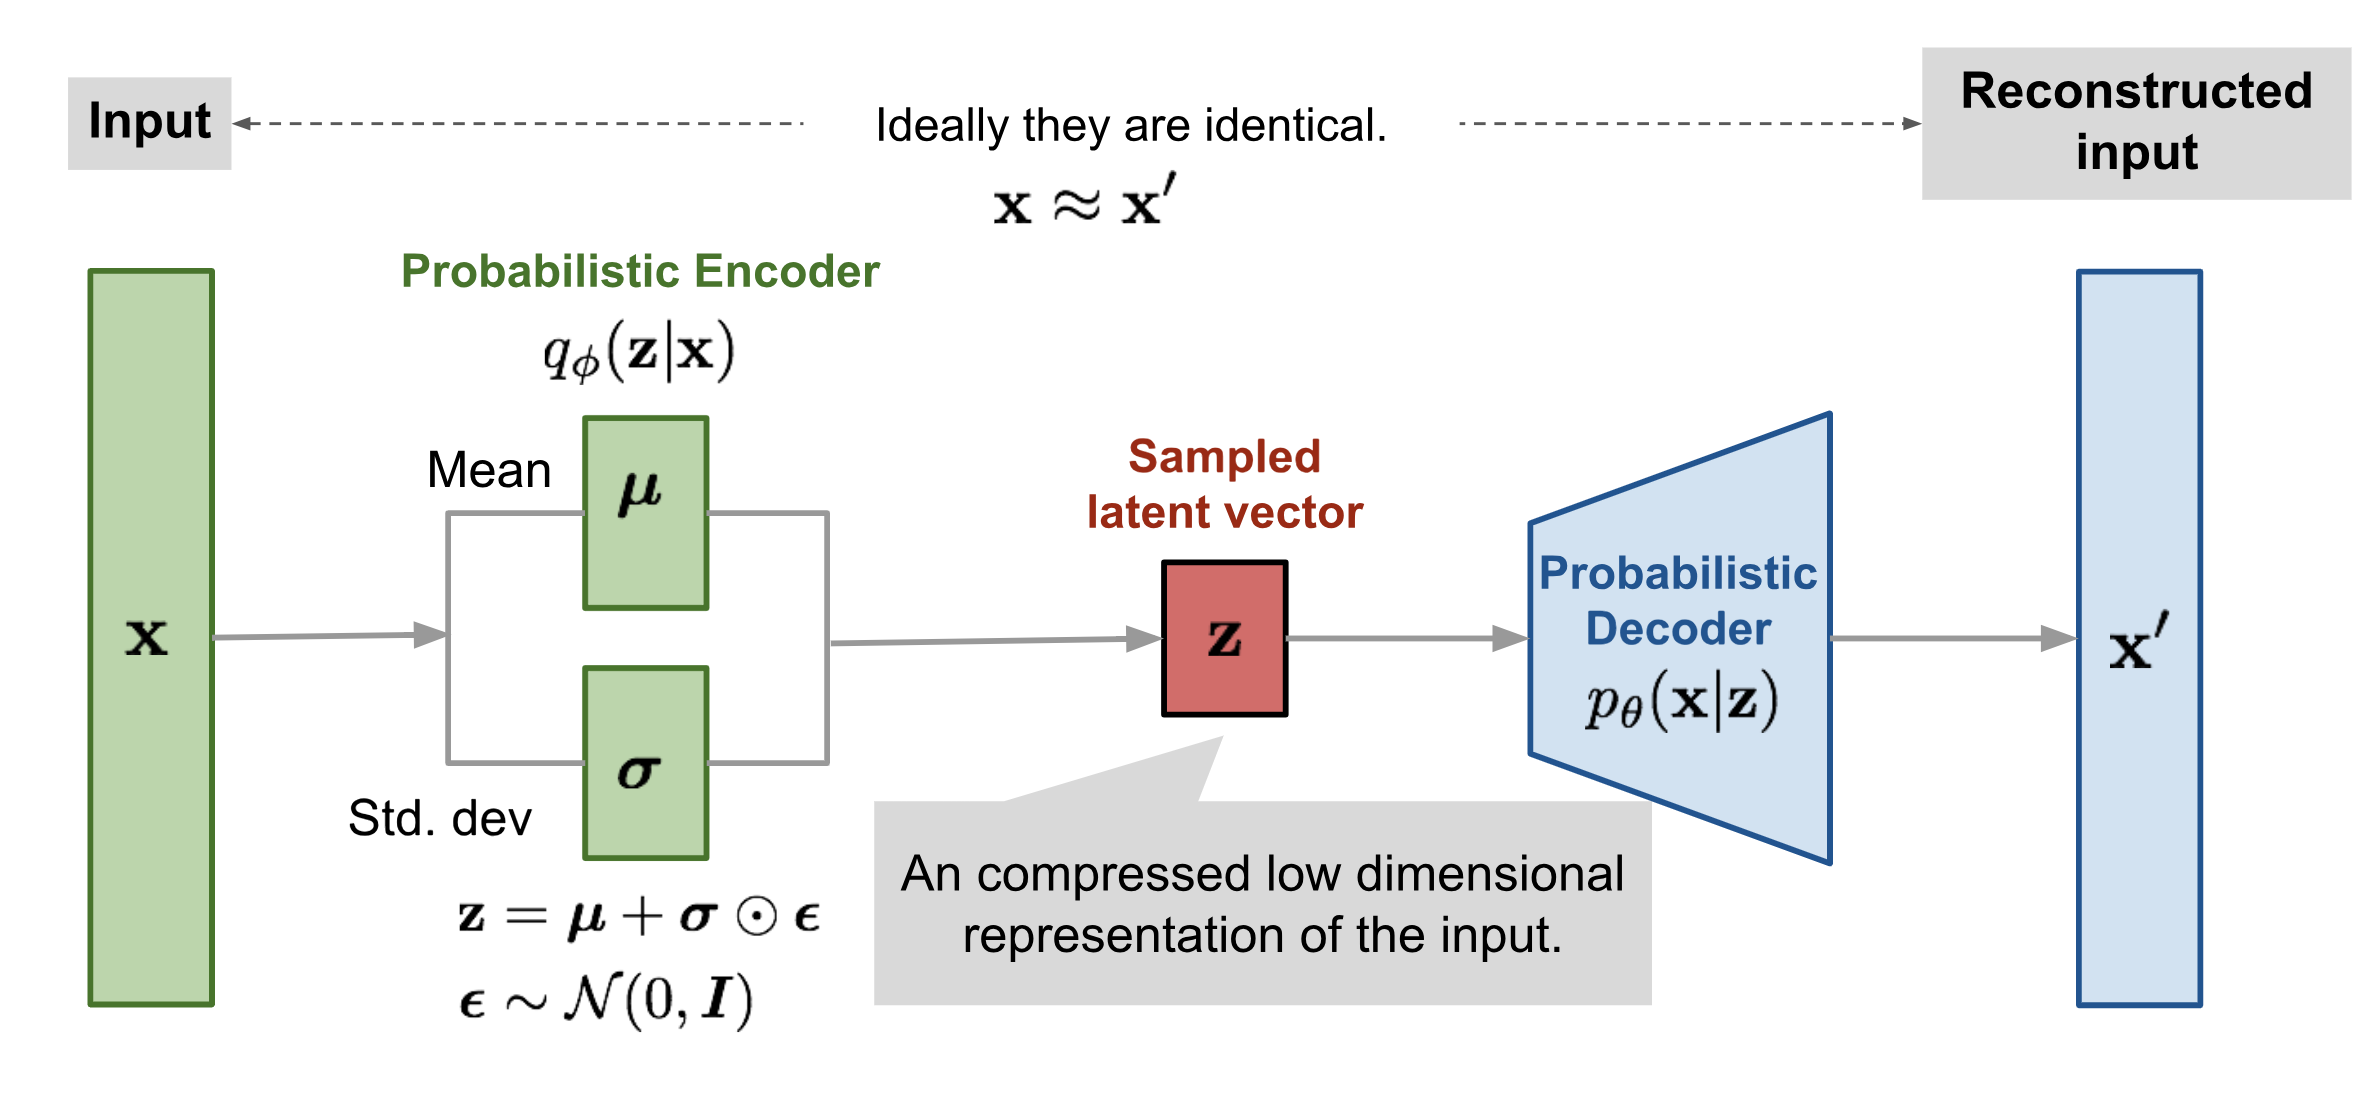
\includegraphics[width=\linewidth]{figs/vae-gaussian.png}
	\end{figure}
	\begin{itemize}
		\item Previous VAE models had \textbf{continuous} latent variables $\bz$.
		\item \textbf{Discrete} representations $\bz$ are potentially a more natural fit for many of the modalities.
		\item Powerful autoregressive models (like PixelCNN) have been developed for modelling distributions over discrete variables.
	\end{itemize}
\end{frame}
%=======
\begin{frame}{Discrete VAE}
	If $\bz$ is a discrete random variable we cannot differentiate through it.
	
	\begin{block}{Gumbel-Max trick}
		Let $G_k \sim \text{Gumbel}$ for $k = 1, \dots, K$, i.e. $G = - \log (\log u)$, $u \sim \text{Uniform}[0, 1]$. Then a discrete random variable
		\vspace{-0.2cm}
		\[
			z = \argmax_k (\log \pi_k + G_k), \quad \sum_k \pi_k = 1
		\]
		\vspace{-0.5cm} \\
		has a categorical distribution $z \sim \text{Categorical}(\bpi)$ ($P(z = k) = \pi_k$).
	\end{block}
	\textbf{Problem:} We still have non-differentiable $\argmax$ operation.
	\begin{block}{Gumbel-Softmax relaxation}
		
		\[
			z_k = \frac{\exp ((\log \pi_k + G_k) / \tau)}{\sum_{j=1}^K \exp ((\log \pi_j + G_j) / \tau)}, \quad k = 1, \dots, K.
		\]
		Here $\tau$ is a temperature parameter.
 	\end{block}
	\myfootnote{
	\href{https://arxiv.org/abs/1611.00712}{Maddison C. J., Mnih A., Teh Y. W. The Concrete distribution: A continuous relaxation of discrete random variables, 2016} \\
	\href{https://arxiv.org/abs/1611.01144}{Jang E., Gu S., Poole B. Categorical reparameterization with Gumbel-Softmax, 2016}
	}
\end{frame}%=======
\begin{frame}{Discrete VAE}
	\vspace{-0.3cm}
	\begin{block}{Gumbel-Softmax relaxation}
		Concrete distribution = continuous + discrete
		\vspace{-0.2cm}
		\[
			z_k = \frac{\exp ((\log \pi_k + G_k) / \tau)}{\sum_{j=1}^K \exp ((\log \pi_j + G_j) / \tau)}, \quad k = 1, \dots, K.
		\]
		\vspace{-0.4cm} \\
		Here $\tau$ is a temperature parameter. Now we have differentiable operation.
 	\end{block}
 	\vspace{-0.2cm}
 	\begin{figure}
 		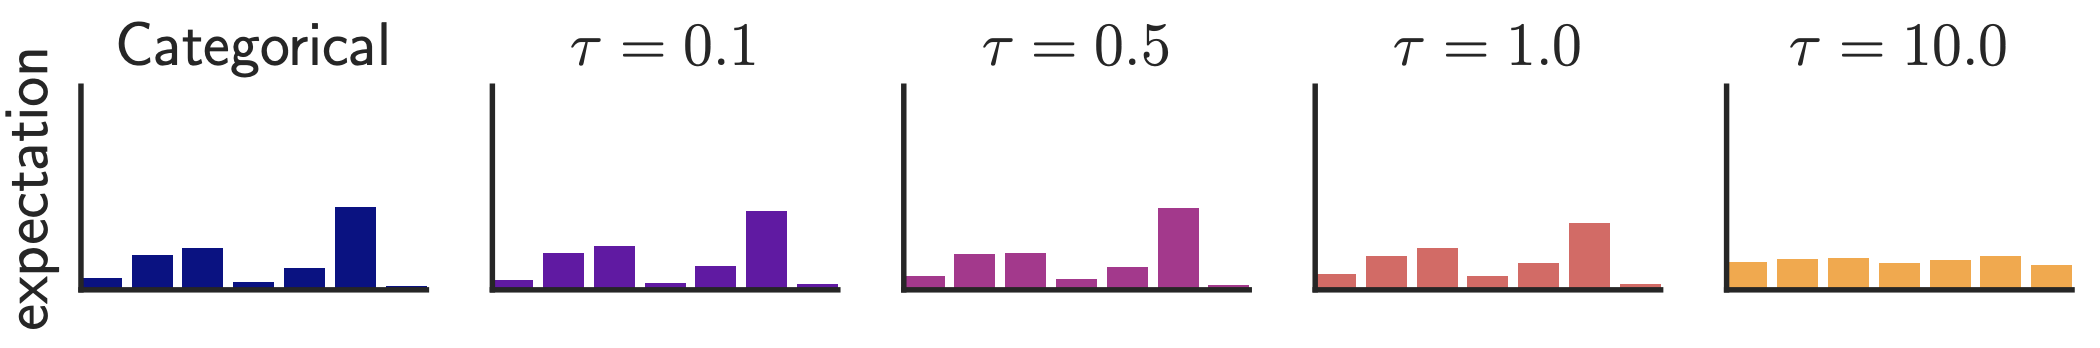
\includegraphics[width=0.8\linewidth]{figs/gumbel_softmax}
 	\end{figure}
 	\vspace{-0.7cm}
 	\begin{figure}
 		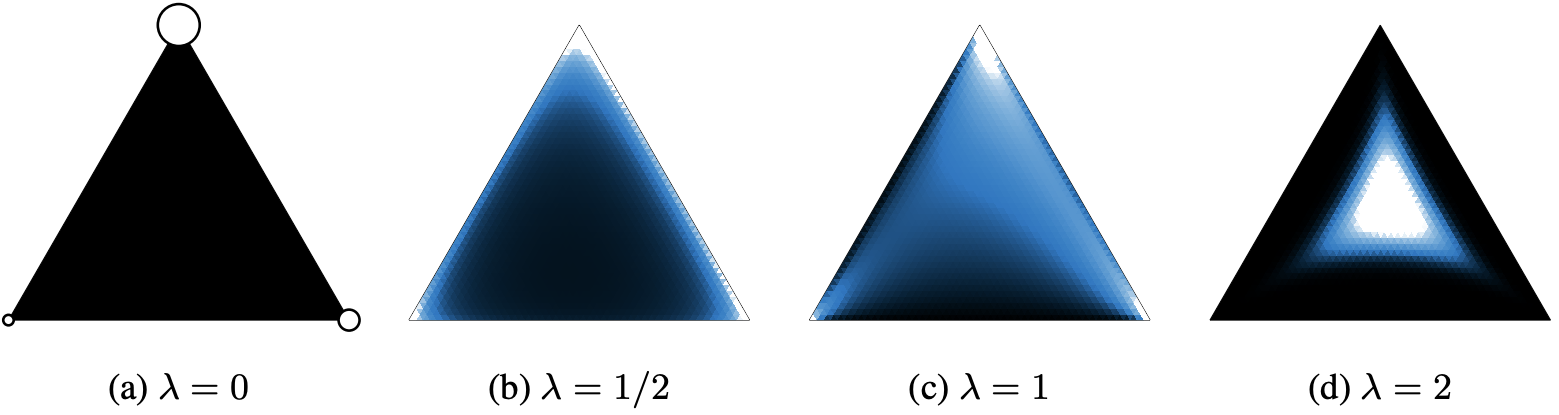
\includegraphics[width=0.8\linewidth]{figs/simplex}
 	\end{figure} 
	\myfootnote{
	\href{https://arxiv.org/abs/1611.00712}{Maddison C. J., Mnih A., Teh Y. W. The Concrete distribution: A continuous relaxation of discrete random variables, 2016} \\
	\href{https://arxiv.org/abs/1611.01144}{Jang E., Gu S., Poole B. Categorical reparameterization with Gumbel-Softmax, 2016}
	}
\end{frame}
%=======
\begin{frame}{Vector Quantized VAE}
	\begin{itemize}
		\item Define dictionary space $\{\be_k\}_{k=1}^K$, where $\be_k \in \bbR^C$, $K$ is the size of the dictionary.
		\item Let $\bz = \text{NN}_\text{e}(\bx) \in \bbR^{W \times H \times C}$ be an encoder output.
		\item Quantized representation $\bz_q \in \bbR^{W \times H \times C}$ is defined by a nearest neighbour look-up using the shared dictionary space for each of $W \times H$ spatial locations
		\vspace{-0.2cm}
		\[
			[\bz_q]_{ij} = \be_{k^*}, \quad \text{where } k^* = \argmin_k \| [\bz_e]_{ij} - \be_k \|.
		\] 
	\end{itemize}
	\vspace{-0.6cm}
	\begin{block}{Quantization procedure}
		\begin{minipage}[t]{0.65\columnwidth}
			\begin{figure}
				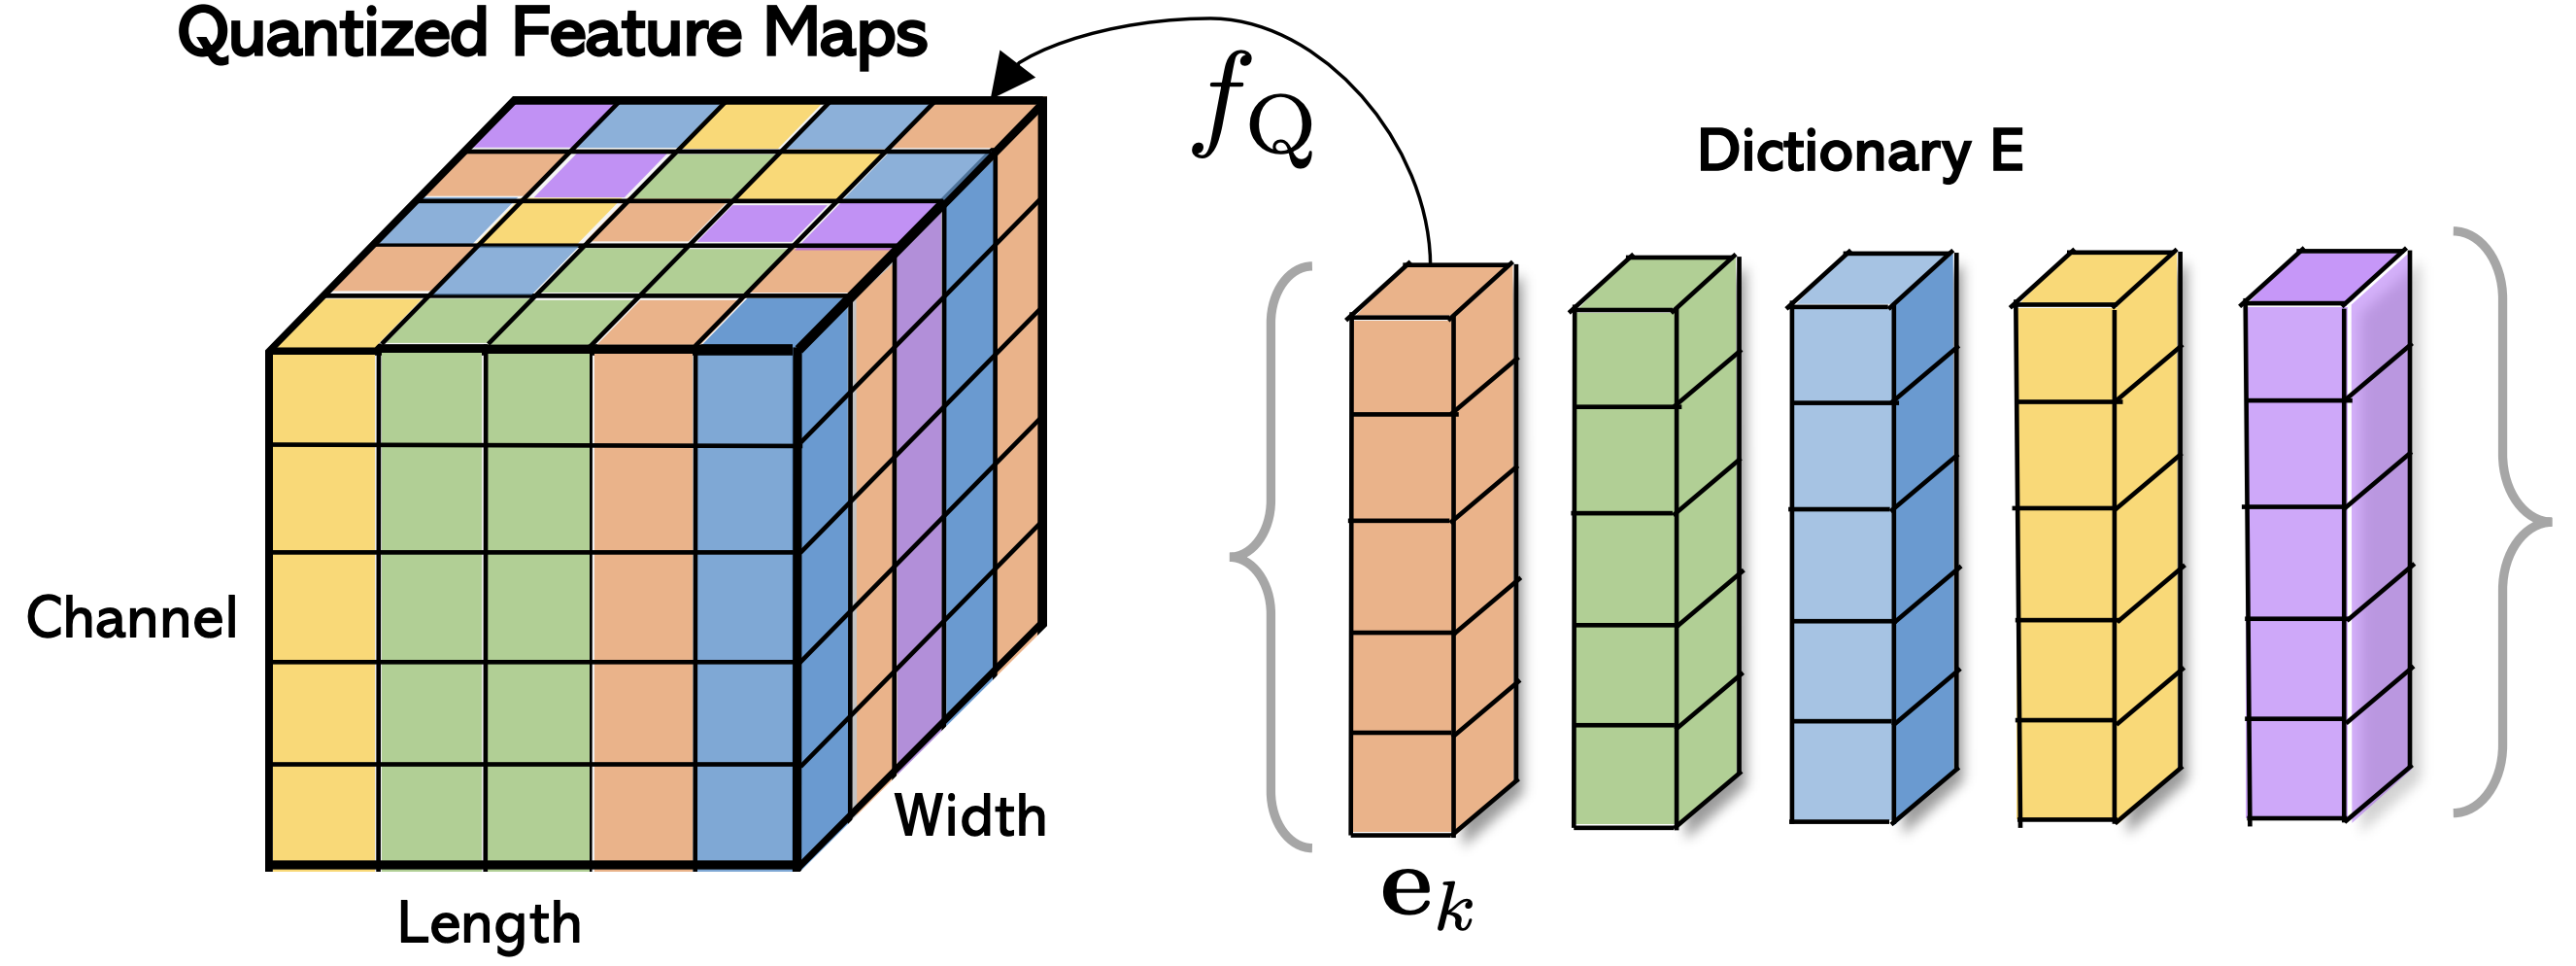
\includegraphics[width=\linewidth]{figs/fqgan_cnn.png}
			\end{figure}
		\end{minipage}%
		\begin{minipage}[t]{0.35\columnwidth}
			\begin{figure}
				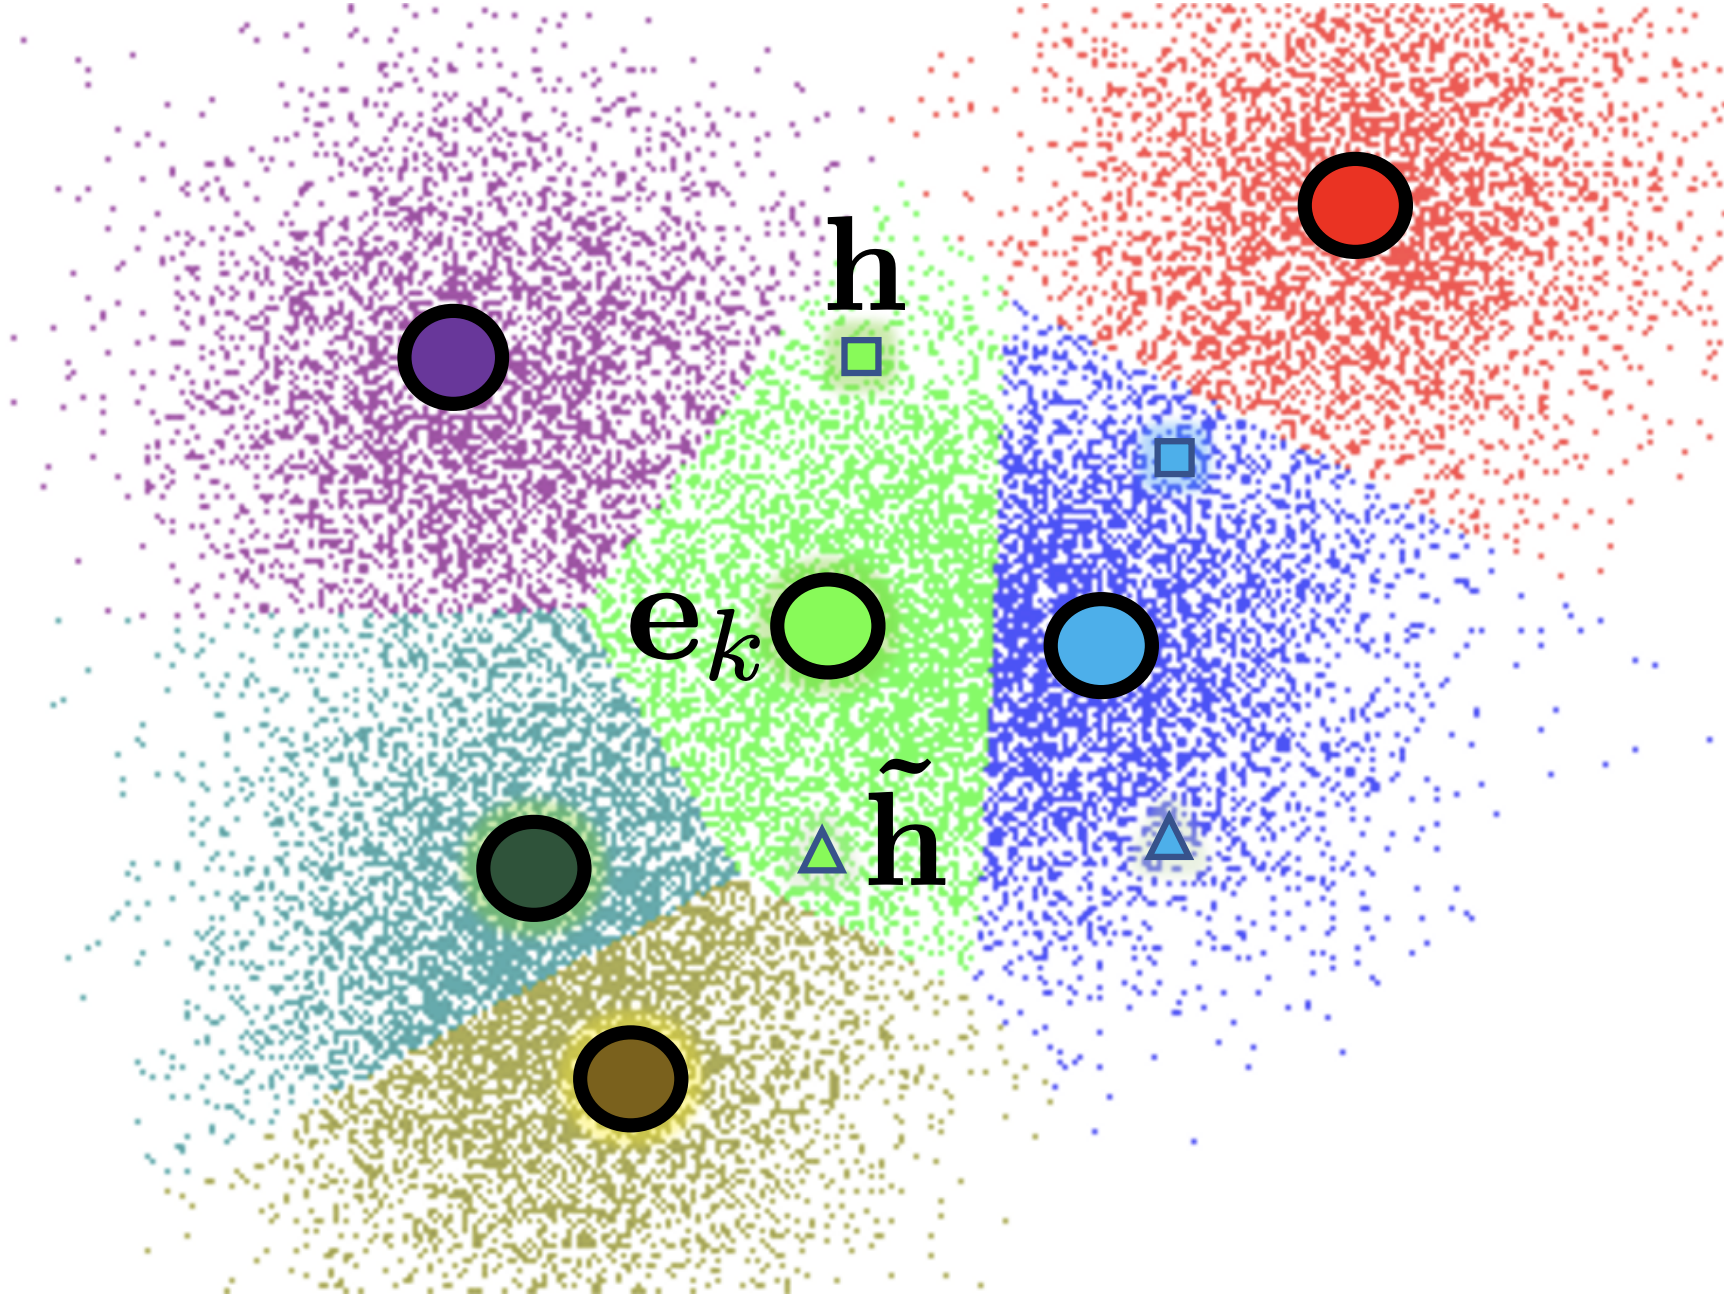
\includegraphics[width=0.9\linewidth]{figs/fqgan_lookup}
			\end{figure}
		\end{minipage}
	\end{block}

	\myfootnotewithlink{https://arxiv.org/abs/2004.02088}{Zhao Y. et al. Feature Quantization Improves GAN Training, 2020} 
\end{frame}
%=======
\begin{frame}{Vector Quantized VAE}
	Define VAE latent variable $\hat{\bz} \in \bbR^{W \times H}$ with prior distribution $p(\hat{\bz}) = \text{Uniform}\{1, \dots, K\}$ and variational posterior distribution 
	\vspace{-0.3cm}
	\[
		q(\hat{\bz} | \bx) = \prod_{i=1}^W \prod_{j=1}^H q(\hat{z}_{ij} | \bx)
	\]
	\vspace{-0.3cm}
	\[
		q(\hat{z}_{ij} = k^* | \bx) = \begin{cases}
			1 , \quad \text{for } k^* = \argmin_k \| [\bz_e]_{ij} - \be_k \| \\
			0, \quad \text{otherwise}.
		\end{cases}
	\]
	\vspace{-0.5cm}
	\begin{block}{ELBO objective}
		\vspace{-0.5cm}
		\[
		 \mathcal{L} (\bphi, \btheta)  = \mathbb{E}_{q(\hat{\bz} | \bx, \bphi)} \log p(\bx | \hat{\bz}, \btheta)] - KL(q(\hat{\bz}| \bx) || p(\hat{\bz})) \rightarrow \max_{\bphi, \btheta}.
		\]	
		\vspace{-0.5cm}
	\end{block}
	\begin{itemize}
		\item VAE proposal distribution $q(\hat{\bz} | \bx)$ is deterministic. 
		\item $KL(q(\hat{z}| \bx) || p(\hat{z}))$ term in ELBO is constant (equals to $\log K$).
	\end{itemize}
	
	\myfootnotewithlink{https://arxiv.org/abs/1711.00937}{Oord A., Vinyals O., Kavukcuoglu K. Neural Discrete Representation Learning, 2017} 
\end{frame}
%=======
\begin{frame}{Vector Quantized VAE}
	\begin{figure}
		\centering
		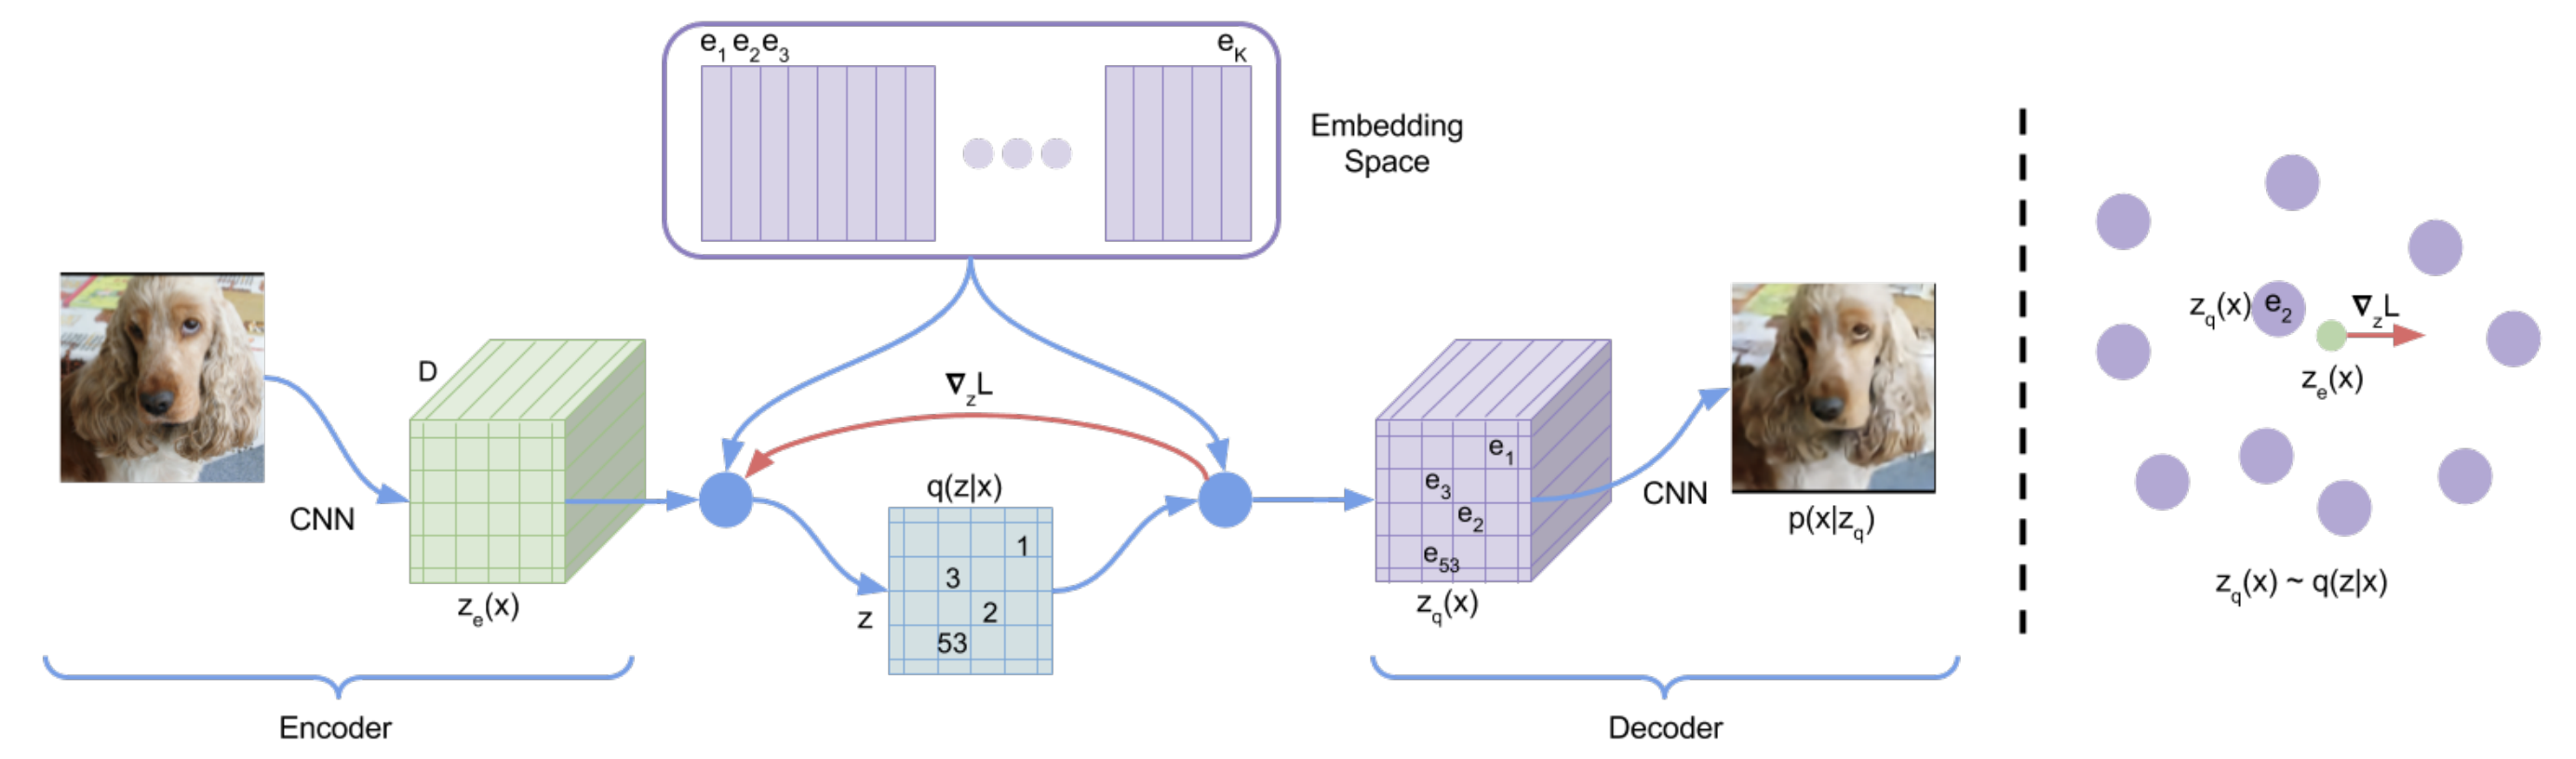
\includegraphics[width=\linewidth]{figs/vqvae}
	\end{figure}
	\begin{block}{Objective}
		\vspace{-0.3cm}
		\[
			\log p(\bx | \bz_q) + \| \text{sg} (\bz_e) - \bz_q \| + \beta \| \bz_e - \text{sg}(\bz_q) \|
		\]
	\end{block}
	\begin{itemize}
		\item First term is ELBO part.
		\item Quantization operation is not differentiable.
		\item Straight-through gradient estimation is used to backpropagate the quantization operation.
	\end{itemize}

	\myfootnotewithlink{https://arxiv.org/abs/1711.00937}{Oord A., Vinyals O., Kavukcuoglu K. Neural Discrete Representation Learning, 2017} 
\end{frame}
%=======
\begin{frame}{Vector Quantized VAE-2}
	\begin{block}{Samples 1024x1024}
		\vspace{-0.2cm}
		\begin{figure}
			\centering
			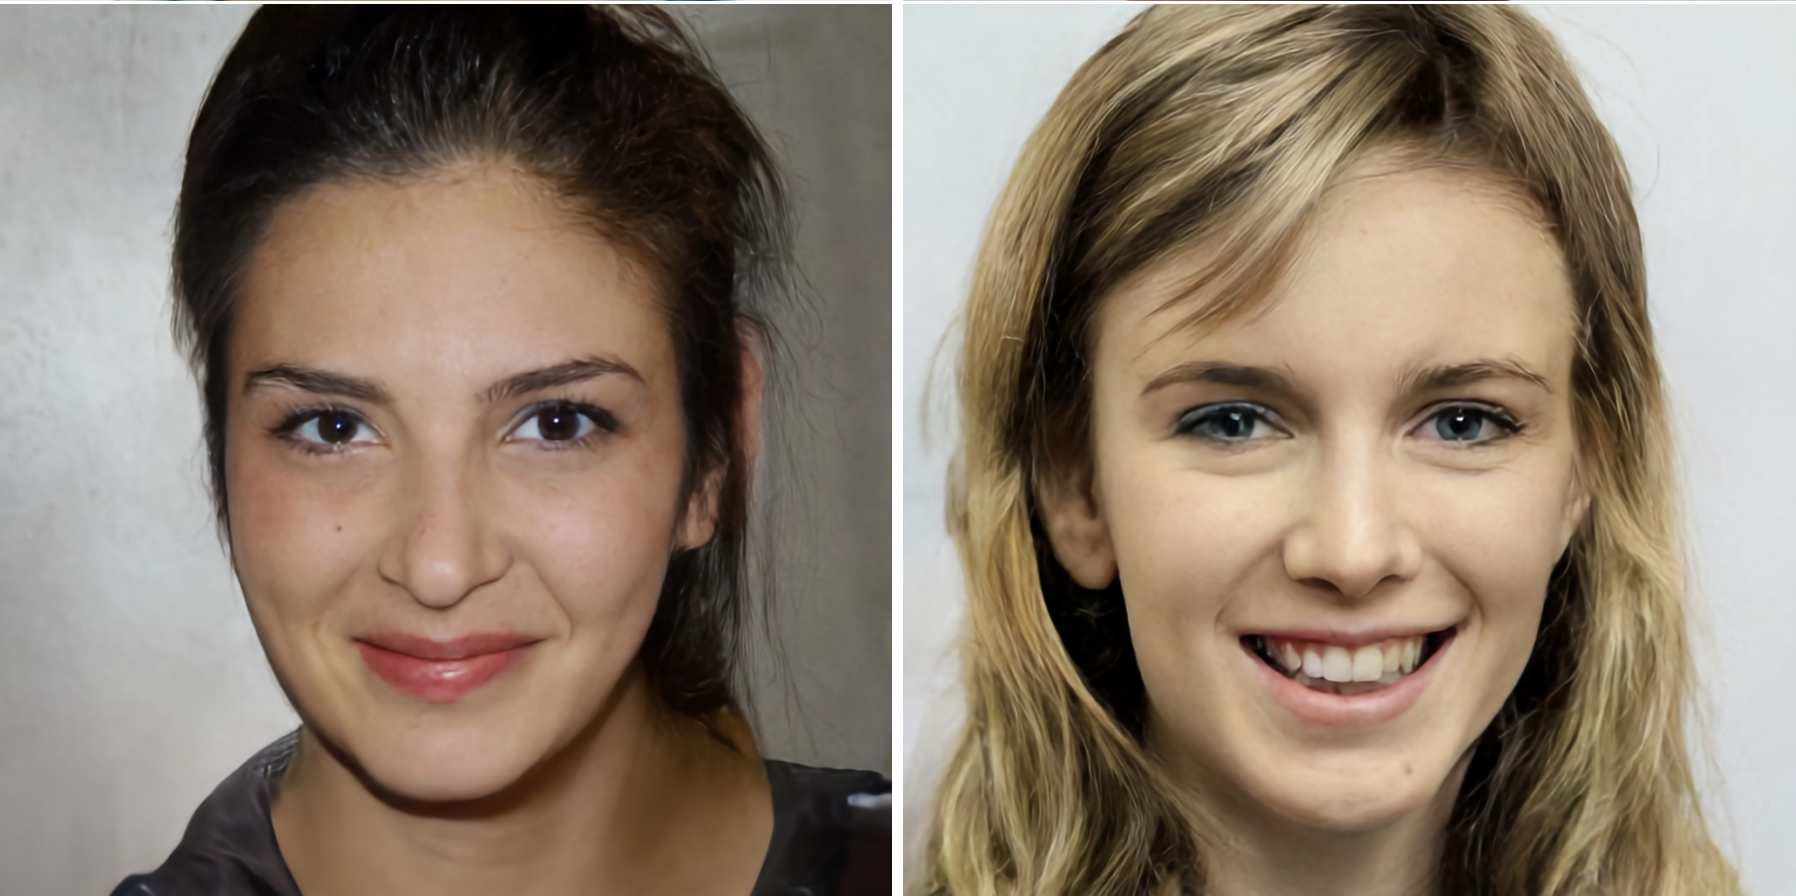
\includegraphics[width=0.63\linewidth]{figs/vqvae2_faces}
		\end{figure}
	\end{block}
	\vspace{-0.6cm}
	\begin{block}{Samples diversity}
		\vspace{-0.2cm}
		\begin{figure}
			\centering
			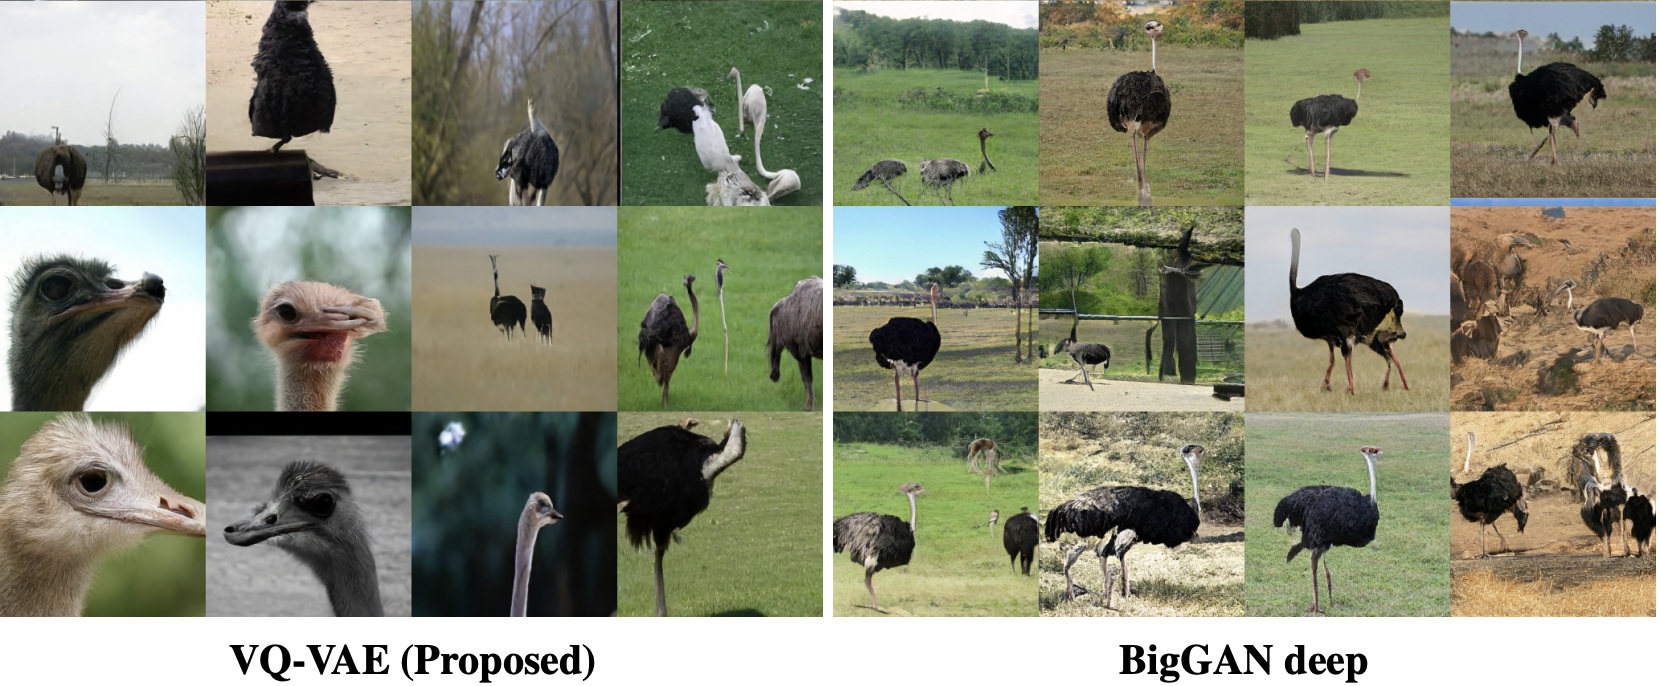
\includegraphics[width=0.65\linewidth]{figs/vqvae2_diversity}
		\end{figure}
	\end{block}
	\myfootnotewithlink{https://arxiv.org/abs/1906.00446}{Razavi A., Oord A., Vinyals O. Generating Diverse High-Fidelity Images with VQ-VAE-2, 2019} 
\end{frame}
%=======
\begin{frame}{DALL-E}
	\begin{block}{Deterministic VQ-VAE posterior}
		\vspace{-0.3cm}
		\[
			q(\hat{z}_{ij} = k^* | \bx) = \begin{cases}
				1 , \quad \text{for } k^* = \argmin_k \| [\bz_e]_{ij} - \be_k \| \\
				0, \quad \text{otherwise}.
			\end{cases}
		\]
		\vspace{-0.3cm}
	\end{block}
	\begin{itemize}
		\item It is possible to use Gumbel-Softmax trick to relax this distribution to continuous one.
		\item Since latent space is discrete we could train autoregressive transformers in it.
		\item It is a natural way to incorporate text and image spaces.
	\end{itemize}
	\begin{figure}
		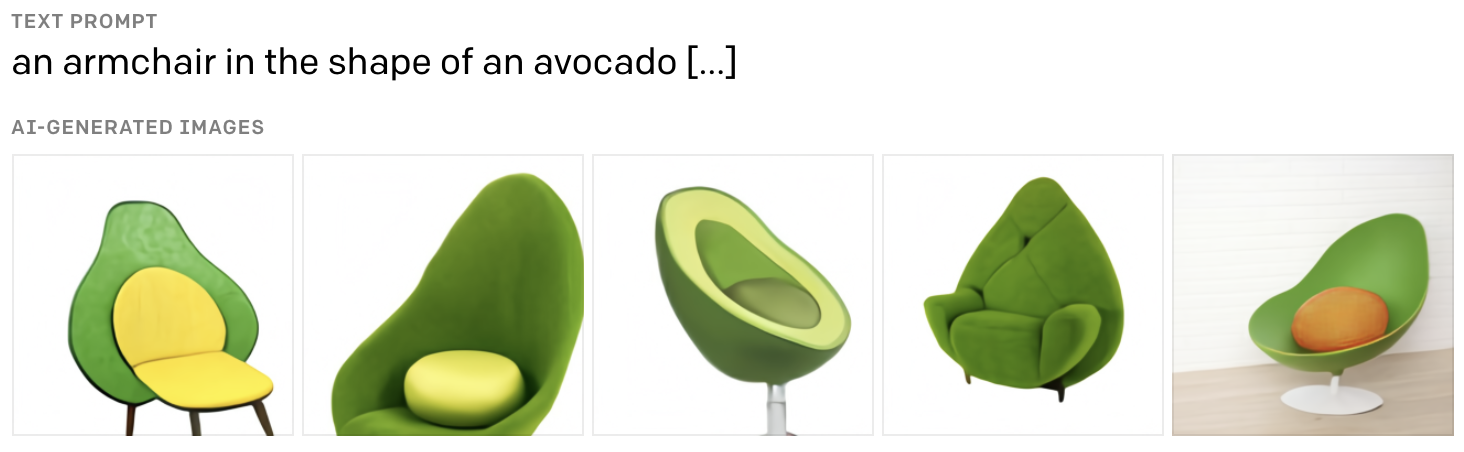
\includegraphics[width=\linewidth]{figs/dalle}
	\end{figure}
	\myfootnotewithlink{https://arxiv.org/abs/2102.1209}{Ramesh A. et al. Zero-shot text-to-image generation, 2021}
\end{frame}
%=======
\begin{frame}{Summary}
	\begin{itemize}
	\item Gumbel-Softmax and Quantization are the two ways to create VAE with discrete latent space.
	\vfill
	\item It becomes more and more popular to use discrete latent spaces in the fields of image/video/music generaton.
	\end{itemize}
\end{frame}
\end{document} 